\section{58 - MAT - AN 1.2, AN 4.3, AN 2.1, FA 2.3, FA 2.2, FA 4.3 - Intercity-Express (ICE) - Matura 2015/16 Haupttermin}

\begin{langesbeispiel} \item[0] %PUNKTE DES BEISPIELS
	
Als ICE werden verschiedene Baureihen von Hochgeschwindigkeitszügen der Deutschen Bahn bezeichnet. Mit einer Höchstgeschwindigkeit von bis zu 330\,km/h (rund 91,7\,m/s) handelt es sich dabei um die schnellsten Züge Deutschlands. Sie sind ca. 200 Meter lang und ca. 400 Tonnen  schwer und bestehen aus jeweils acht Wagen. Im Rahmen von Zulassungsfahrten müssen Beschleunigungs- und Bremstests absolviert werden. Ergebnisse dieser Tests können grafisch dargestellt werden. 

\subsection{Aufgabenstellung:}
\begin{enumerate}
	\item Die Daten eines Beschleunigungstests vom Stillstand bis zur Höchstgeschwindigkeit (die Geschwindigkeit $v_1(t)$ ist in Metern pro Sekunde und die Zeit $t$ in Sekunden angegeben) sind im nachstehenden Zeit-Geschwindigkeit-Diagramm näherungsweise dargestellt.
	
	\begin{center}
	\resizebox{0.8\linewidth}{!}{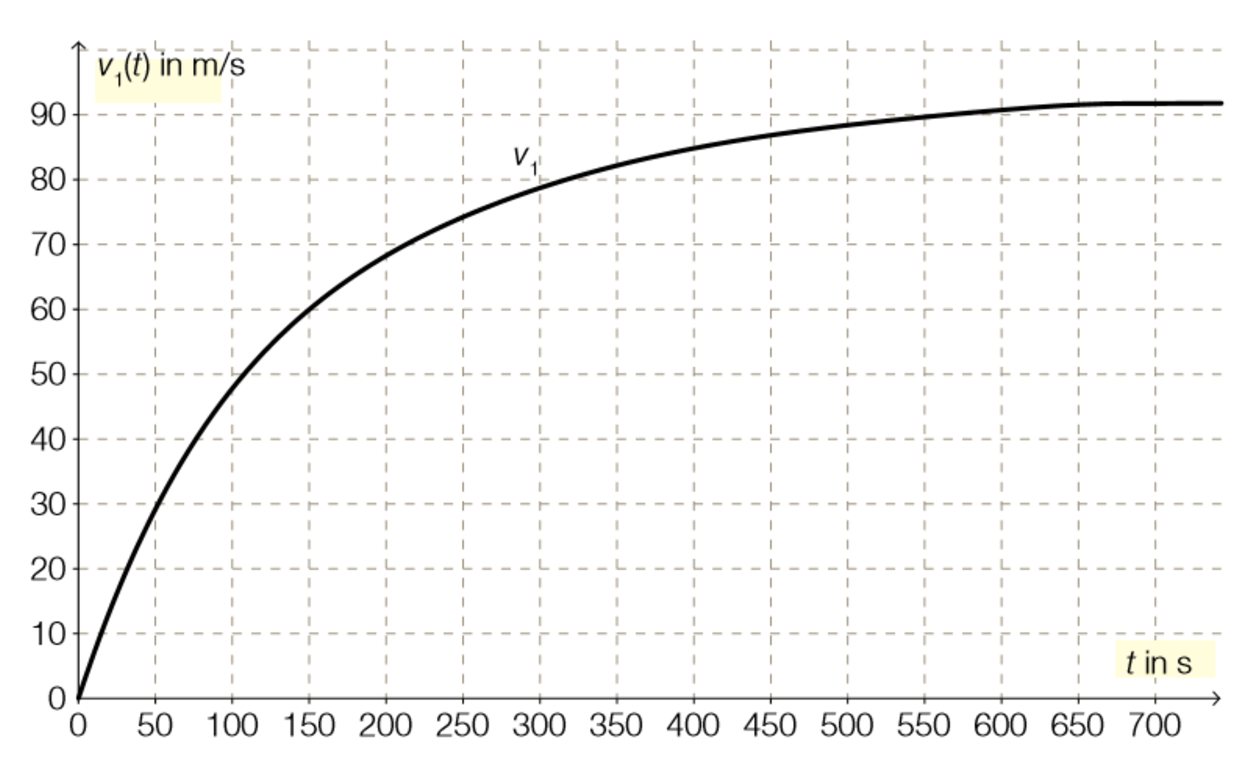
\includegraphics{../_database/Bilder/Bild58-1.eps}}
\end{center}

Bestimme die mittlere Änderungsrate der Geschwindigkeit im Zeitintervall $[0\,\text{s};700\,\text{s}]$ und gib einen Zeitpunkt an, zu dem die momentane Änderungsrate der Geschwindigkeit größer ist als die ermittelte mittlere Änderungsrate!\leer

\fbox{A} Interpretiere das bestimmte Intergral $\int^{700}_0{v_1(t)}$d$t$ im gegebenen Kontext!\leer

\item Bei einem Bremstest werden Daten aufgezeichnet. Diesen Daten kann man für den zurückgelegten Weg $s(t)$ entnehmen: $s(t)=70\cdot t-0,25\cdot t^2$ mit $t$ in Sekunden und $s(t)$ in Metern ab Bremsbeginn.\leer

Gib die Zeit-Geschwindigkeit-Funktion $v_2$ für den Bremstest in Form von $v_2(t)=k\cdot t+d$ an und deute die auftretenden Parameter $k$ und $d$ im gegebenen Kontext!\leer

Bestimme die Länge derjenigen Strecke, die der ICE vom Bremsbeginn bis zum Stillstand zurücklegt!
						\end{enumerate}\leer
				
\antwort{
\begin{enumerate}
	\item \subsection{Lösungserwartung:} 
	
mittlere Änderungsrate: 0,131\,m/s$^2$

möglicher Zeitpunkt für die momentane Änderungsrate: $t=150$\,s\leer

Der Wert des angegebenen bestimmten Integrals entspricht dem im Zeitintervall $[0\,\text{s}; 700\,\text{s}]$ zurückgelegten Weg (in Metern).

	\subsection{Lösungsschlüssel:}
	\begin{itemize}
		\item Ein Punkt für die Angabe sowohl einer korrekten mittleren Änderungsrate als auch eines entsprechenden Zeitpunkts, wobei die Einheiten "`m/s$^2$"' bzw. "`s"' nicht angeführt sein  müssen. 
		
		Toleranzintervall für die mittlere Änderungsrate: $[0,130\,\text{m/s}^2; 0,133\,\text{m/s}^2]$ 
		
		Toleranzintervall für den Zeitpunkt: $[0\,\text{s}; 230\,\text{s}] $
		\item Ein Ausgleichspunkt für eine (sinngemäß) korrekte Interpretation.
	\end{itemize}
	
	\item \subsection{Lösungserwartung:}
			
	$v_2(t)=70-0,5\cdot t$\leer
	
	Mögliche Deutungen von $k$:
	
	Die Geschwindigkeit nimmt während des Bremsvorgangs in jeder Sekunde (konstant) um $0,5$\,m/s ab.\leer
	
	oder:
	
	Die Beschleunigung (ist konstant und) beträgt $-0,5$\,m/s$^2$.\leer
	
	oder:
	
	Die Verzögerung durch das Bremsen (ist konstant und) beträgt 0,5\,m/s$^2$.\leer
	
	Mögliche Deutung von $d$:
	
	Die Geschwindigkeit zu Beginn des Bremsvorgangs beträgt 70\,m/s.
	
	$v_2(t)=0 \Rightarrow t=140$\,s $\Rightarrow s(140)=4\,900$\,m

	\subsection{Lösungsschlüssel:}
	
\begin{itemize}
	\item Ein Punkt für eine korrekte Gleichung und eine (sinngemäß) korrekte Deutung beider Parameter. Äquivalente Gleichungen sind als richtig zu werten. 
	\item Ein Punkt für die richtige Lösung, wobei die Einheit "`m"' nicht angeführt sein muss.
\end{itemize}

\end{enumerate}}
		\end{langesbeispiel}